\chapter{电分析化学}

电化学是研究化学能和电能相互转化的化学领域。电分析化学是使用电化学技术来表征
样品的方法。电化学,电重力法和极谱法的最初分析应用是定量测定水溶液中的痕量金属
。后一种方法可靠且灵敏,足以检测许多金属中低至1 ppm的浓度。从那时起,出现了许多
不同类型的电化学技术,每种技术都可用于有机,无机和生物化学分析中的特定应用。

在施加电压或电流时发生还原或氧化的物质称为电活性物质。通常,在水或非水溶剂中
甚至在薄膜中,电活性物质可以是溶剂化或络合的离子或分子。现在,电化学方法不仅
用于痕量金属离子分析,还用于有机化合物的分析,连续过程分析以及研究单个活细胞内
的化学反应。已经开发了适用于工业中产品流质量控制,体内监测,材料表征以及制药和
生化研究的应用程序,其中仅举几例。在正常条件下,可以轻松确定低至1 ppm的浓度。
通过使用电沉积,然后反转电流或电势,可以将许多电活性物质的灵敏度极限扩展三到四
个数量级,从而提供了ppb级的分析手段。

在实践中,电化学不仅提供元素和分子分析,还可以用于通过极谱法,电流分析法,电导
分析法和电位计研究获得关于平衡,动力学和反应机理的信息。分析计算通常基于电流或
电压的确定,或者基于电池在一定条件下产生的电阻,这些条件取决于所研究物质的浓度。
电化学测量很容易实现自动化,因为它们是电信号。该设备通常比光谱仪器便宜得多。
\section{电化学基础}
电化学是对还原-氧化反应(称为氧化还原反应)的研究,其中电子从一种反应物转移到
另一种反应物。在氧化还原反应中失去电子的化学物质被氧化。获得电子的物质被还原。
被氧化的物质也被称为还原剂,因为它会导致其他物质被还原。同样,氧化剂是在反应中
本身被还原的物质。氧化还原反应要求一种反应物从被氧化的反应物中获得电子(被还原
)。我们可以将还原反应和氧化反应分别写为半反应;半反应的总和等于净氧化还原反应
。氧化半反应的例子包括
\begin{center}
    \ce{Fe^{2+} -> Fe^{3+} + e^{-}}\\
    \ce{Cu(s) -> Cu^{2+} + 2e^{-}}\\
    \ce{AsH3(g) -> As(s) + 3H+ + 3e^-}\\
    \ce{H2C2O4 -> 2CO2(g) + 2H+ + 2e^-}
\end{center}
还原半反应例子包括
\begin{center}
    \ce{Co^{3+} + e^{-} -> Co^{2+}}\\
    \ce{IO3^{-} + 6H+ + 5e^{-} -> 1/2 I2(s) + 3 H2O}\\
    \ce{Cl2(g) + 2e^{-} -> 2Cl-}\\
    \ce{Ag+ + e- -> Ag(s)}
\end{center}
把一个氧化反应反向书写,它变成还原,比如,\ce{Al^{3+}}接受3个电子,还原为\ce{Al}。
所有还原反应都是氧化反应的反方向。正如我们所见,实际上,很多这样的反应都是
可逆的。

一个实际的氧化还原反应是一个氧化半反应和还原半反应之和。半反应需要乘以系数,以
确保氧化还原总反应没有电子出现。例如\ce{Cu}、\ce{Cu^{2+}}、\ce{Ag}和\ce{Ag+}之间
的反应
\begin{center}
    \ce{Cu(s) + 2Ag+ -> Cu^{2+} + 2Ag(s)}
\end{center}
对应的半反应为
\begin{center}
    \begin{tabular}{rl}
        氧化反应:&\ce{Cu(s) -> Cu^{2+} + 2e-}\\
        还原反应:&\ce{Ag+ + e- -> Ag(s)}\\
    \end{tabular}
\end{center}
1 mol铜给出2 mol电子,而1 mol银离子只能接受1 mol电子。因此,将还原反应乘以2,
这样,两个半反应之和,就没有电子形式:
\begin{center}
    \begin{tabular}{rl}
        氧化反应:&\ce{Cu(s) -> Cu^{2+} + 2e-}\\
        还原反应:&\ce{2(Ag+ + e- -> Ag(s))}\\
        总反应:&\ce{Cu(s) + 2Ag+ -> Cu^{2+} + 2Ag(s)}\\
    \end{tabular}
\end{center}

电化学反应在电化学池中进行,电化学池是电路的一部分,可以测量电子转移、电流和
电压。这些参数都能提供给我们氧化还原反应的信息,理解电荷、电流和电压之间的关系
是至关重要的。一个电子电量的绝对值是$1.602\times 10^{-19}$库仑(C);这是电子电荷
的基本单位,那么,1 mol电子所带电量为
\begin{equation}
    (1.602\times 10^{-19} \text{ C}/e^-)(6.022\times 10^{23} e^-/\text{mol})
    = 96485 \text{ C/mol}
    \label{15.1}
\end{equation}
96485 C/mol称为法拉第常数($F$),$n$ mol电子总电量$q$为
\begin{equation}
    q = n\times F
    \label{15.2}
\end{equation}
电路中,每秒流过的电量为电流($i$),电流的单位是安培,符号$A$,$1A = 1 C/s$。
电势差$E$,是电化学池内两点间电荷移动所需的能量。如果电子从第一点吸引到第二点,
电子做功。如果第二点排斥电子,那么第二点做功。功的单位为焦耳($J$),电势差$E$的
单位为伏特($V$),功与电势差关系为
\begin{equation}
    w (J) = E (V) \times q (C)
    \label{15.3}
\end{equation}
$1 V = 1 J/C$。

电路中,电流和电势差遵循Ohm定律
\begin{equation}
    i=\frac{E}{R}
    \label{15.4}
\end{equation}

\section{电化学池}
电化学池是电化学的核心部件。我们从连接两个半电池来建立电化学池。当将金属条浸入
合适的离子溶液(一般为该金属离子溶液)中时,在金属和溶液之间产生电势差(电压),
构成半电池,或电极,见图\ref{fig:15.1}。溶液中的金属称为{\bf 电极(electrode)},
离子溶液称为{\bf 电解质(electrolyte)}。我们使用电极一词,来表示半电池中的固体
电导体和整个情况下的完整的半电池,例如,标准氢电极(SHE)和甘汞电极。每个半电池
都有自己的特征电势差或\emph{电极电势(electrode potential)}。电极电势测量半电池
做功的能力或半电池反应的驱动力。金属于离子之间的反应可表示为:
\begin{figure}[htpb]
    \centering
    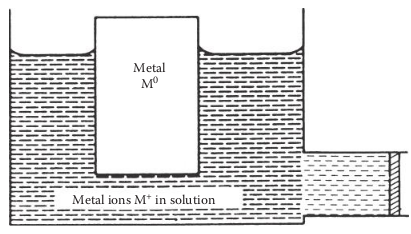
\includegraphics[width=0.65\textwidth]{2021-01-28_17-01.png}
    \caption{半电池示意图}
    \label{fig:15.1}
\end{figure}
\begin{equation}
    M^0 \rightarrow M^{n+} + ne^-
    \label{15.5}
\end{equation}
金属原子失去电子数目$n$是一个整数,金属失去电子,这是氧化反应,中性金属变成
阳离子。该反应中,金属离子进入溶液。发生氧化反应的电极,定义为{\bf 阳极(anode)}
。

这类半电池形如:
\begin{center}
    \begin{tabular}{l}
        \ce{Cd(s) -> Cd^{2+} + 2e^-}\\
        \ce{Ag(s) -> Ag^+ + e^-}\\
        \ce{Cr(s) -> Cr^{3+} + 3e^-}\\
    \end{tabular}
\end{center}
通常情况下,中性金属氧化态为0,不标记。有些金属逆反应是自发的,即金属离子得到
电子变成中性金属。可写作
\begin{equation}
    M^{n+} + ne^- \rightarrow M^{0} 
    \label{15.6}
\end{equation}
发生还原反应。中性金属原子沉积在电极上,称为\emph{电沉积(electrodeposition)},
该电极称为{\bf 阴极(cathode)}。在阴极上,{\bf 电活性物质(electroactive species)
}被还原。电活性物质在反应过程中发生了氧化或还原反应。电化学池也包含非电活性物质
(惰性),如调节电荷平衡的反离子、不参与反应的导电电极。经常使用惰性电极,如
铂或石墨,仅仅在半反应池传导电子进出。

直接测量单一半电池的电势差是不可能的。可以如图\ref{fig:15.2}用两个半电池组成
一个完整电池。一个半电池是铜电极插入\ce{CuSO4}水溶液中,另一个是锌插入\ce{
ZnSO4}水溶液中。半反应和自发反应如下:
\begin{center}
    \begin{tabular}{rl}
        阳极(氧化)反应:&\ce{Zn(s) -> Zn^{2+} + 2e^-}\\
        阴极(还原)反应:&\ce{Cu^{2+} + 2e^- -> Cu(s)}\\
        总反应:&\ce{Zn(s) + Cu^{2+} -> Zn^{2+} + Cu(s)}\\
    \end{tabular}
\end{center}
除非电路闭合,否则不会发生反应,也不会有电流流过。导线通过电压表(电位计)从
外部连接电极。盐桥是在琼脂凝胶中充满饱和\ce{KCl}的玻璃管,物理上,把两种电解质
溶液分开。盐桥允许离子运动完成回路,同时不允许电解质混合。我们需要防止电解质
混合的原因是,我们希望通过测量流经外部电线的电流来获得有关电化学系统的信息。
如果我们将两个电极和两种离子溶液都放在同一容器中,则铜离子将直接在\ce{Zn}电极
上反应,产生相同的反应,但外部电路中没有电流流动。在电解质溶液和盐桥中,电流为
离子(离子运动),而在外部电路中,电流为电子(电子运动)。该电池和图\ref{
fig:15.3}中的电池显示了电化学电池所需的组件:两个电子导体(电极),合适的电解质
溶液以及允许离子在溶液之间移动的装置(图\ref{fig:15.2}是盐桥,图\ref{fig:15.3}
半渗透的玻璃料或膜),通过导线的电极外部连接以及在一个电极上发生氧化反应的能力,
以及在另一个电极上发生还原反应的能力。当然,每种溶液中都存在反离子(例如
硫酸根离子)以平衡电荷。这些离子不是电活性的,也不参与氧化还原反应。它们确实
流动(离子运动)以保持电池中的电荷平衡。使用自发的氧化还原反应发电的电池称为
{\bf 原电池(galvanic cell)}。电池是原电池的例子。设置为通过向电池内通电而引起
非自发反应的电池称为{\bf 电解池(electrolytic cell)}。
\begin{figure}[htpb]
    \centering
    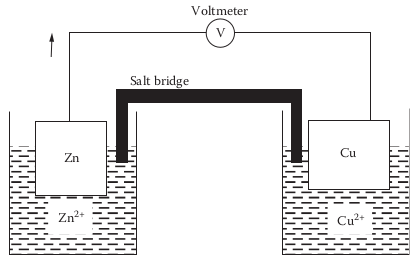
\includegraphics[width=0.65\textwidth]{2021-01-29_16-15.png}
    \caption{Zn/Cu原电池(盐桥)}
    \label{fig:15.2}
\end{figure}
\begin{figure}[htpb]
    \centering
    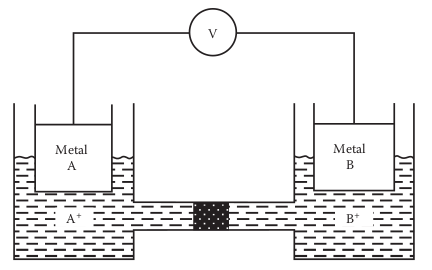
\includegraphics[width=0.65\textwidth]{2021-01-29_16-17.png}
    \caption{半透膜原电池}
    \label{fig:15.3}
\end{figure}

电池具有电势差,即电池电势,通过电压表测量。电池电势差$E_{\text{电池}}$是两个
电极电势之差,两个半电池都写成还原形式。
\begin{equation}
    E_{\text{电池}}=\varphi_{\text{阴极}} - \varphi_{\text{阳极}}
    \label{15.7}
\end{equation}
即使阳极发生的是氧化反应,电位也是还原电位,这一约定保证了计算$E_{\text{电池}}$
的正确性。电池电势也称{\bf 电动势(electromotive force, emf)}。

虽然不能直接测量单电极电势,但是我们可以轻松地测量,如上所述连接的两个半电池
的电势。 我们有了一种通过将半电池连接到指定{\bf 参比电极(reference electrode)}
上来测量其相对电极电势的方法。在实际电池中,还有另一个导致$E_\text{cell}$的
电位差,称为结电位。如果两个半电池的离子浓度或离子类型不同,则在膜或盐桥与溶液
的连接处会产生较小的电势。结电位可能是误差的来源。当使用\ce{KCl}盐桥时,结电势
非常小,因为\ce{K+}和\ce{Cl-}离子的扩散速率相似,因此测量给定电极电势的误差很小。 
\subsection{电池写法}
写出所有的反应,对于电池的写法是耗时的,推荐使用一种简单的写法。如,银电极浸入
0.0001 M \ce{Ag+}水溶液中形成半电池,可写作
\begin{center}
    \ce{Ag(s)|Ag^{+}(0.0001 M)}
\end{center}
\ce{Ag}和\ce{Ag^{+}}之间的竖线表示\emph{相的界面(phase boundary)},图\ref{fig:15.2}
完整电池的写法为
\begin{center}
    \ce{Zn(s)|Zn^{2+}(0.01 M)||Cu^{2+}(0.01 M)|Cu(s)}
\end{center}
双竖线表示结膜或盐桥,作为两个半电池的分割。也可以写成盐的形式:
\begin{center}
    \ce{Zn(s)|ZnSO4(aq)||CuSO4(aq)|Cu(s)}
\end{center}
左侧为阳极,右侧阴极,表示电子流从阳极到阴极。
\subsection{标准还原电势}
\subsubsection{标准氢电极}
为了编制电极电势表,必须将用作参比电极的半电池达成一致。参比电极的电极电势可以
设置成任意值,设置成0是方便的。实践中,规定在所有温度下,标准氢电极的电极电势
为0,如图\ref{fig:15.4}所示。由一个Pt电极组成,该电极的表面涂层为海绵状的铂,
浸入1 M盐酸溶液中,该溶液解离生成\ce{H+}。\ce{H2}在Pt电极上进入酸性溶液。Pt电
极表面上的细碎铂为反应提供了较大的表面积
\begin{equation}
    2H^+ + 2e^- \rightarrow H_2(g)\qquad \varphi^\minuso = 0.000 V
    \label{15.8}
\end{equation}
\begin{figure}[htpb]
    \centering
    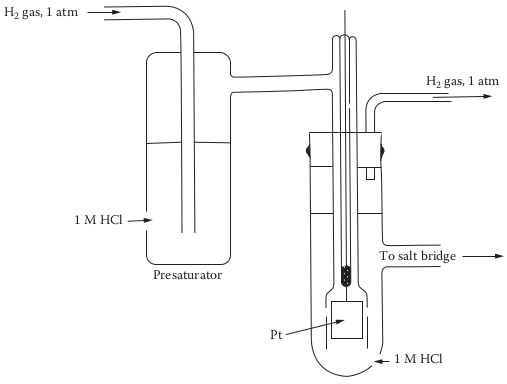
\includegraphics[width=0.75\textwidth]{2021-01-29_19-20.png}
    \caption{标准氢电极}
    \label{fig:15.4}
\end{figure}
另外,Pt用作外部电路的电导体。在标准状态下,即,当\ce{H2}压力等于1个大气压,
且\ce{HCl}的理想浓度为1 M,并且系统处于25 $^\circ$C时,公式\ref{15.8}中给出的
反应的还原电位正好为0V。(电势实际上取决于\ce{HCl}的化学活性,而不是其浓度。
随后讨论了活性和浓度之间的关系。对于理想的溶液,浓度和活性相等。)电势由$E^\minuso$
表示,其中上标表示标准状态条件。术语标准还原电位是指所有溶质的理想浓度为1 M,
所有气体的浓度为1 atm。存在的其他固体或液体是纯净的(例如,纯Pt固体)。通过将
SHE半电池与任何其他标准半电池连接并测量所产生的电压差,我们可以确定第二半电池
所产生的标准还原电位。

例如,25 $^\circ$C时,电池
\begin{center}
    \ce{Zn(s) | Zn^{2+} (aq, 1 M) || H^+ (aq, 1 M) | H_2 (g, 1 atm) | Pt(s)}
\end{center}
\ce{Zn}半电池作为阳极,标准氢电极作为阴极。所有溶液浓度都是理想的1 M,气体的
压力是1 atm,两个半电池都是标准态。测量电池电动势为$+0.76 V$,这是标准电池电势
$E^\minuso$。依据公式\ref{15.7}
\begin{equation}
E^\minuso_\text{电池}=\varphi^\minuso_\text{阴极}-\varphi^\minuso_\text{阳极}
\label{15.9}
\end{equation}
总压是$+0.76V$,标准氢电极是$0V$,所以\ce{Zn}标准还原电位
\[
    +0.76 V = 0.000 - \varphi^\minuso_\text{Zn}
\]
\[
    \varphi^\minuso_\text{Zn} = - 0.76 V
\]
写作
\[
    Zn^{2+} + 2e^- \rightarrow Zn(s) \qquad \varphi^\minuso_\text{Zn}=-0.76 V
\]
即使我们建立的原电池是将\ce{Zn}氧化,依然可以得到还原电位。通过代替其它半电池,
我们可以得到一系列的标准还原电位,并建立电势表。如果我们用标准氢电极和\ce{Cu}
建立一个原电池,标准氢电极做阳极,发生自发反应,电池为
\begin{center}
    \ce{Pt(s) | H_2 (g, 1 atm) | H^+ (aq, 1 M) || Cu^{2+} (aq, 1 M) | Cu(s)}
\end{center}
测得电动势为$+0.34V$,\ce{Cu}标准还原电位为
\[
    +0.34 V = \varphi^\minuso_\text{Cu} - 0.000 V
\]
\[
    \varphi^\minuso_\text{Cu} = + 0.34 V
\]
